%% LyX 2.0.3 created this file.  For more info, see http://www.lyx.org/.
%% Do not edit unless you really know what you are doing.
\documentclass[10pt]{beamer}\usepackage[]{graphicx}\usepackage[]{color}
%% maxwidth is the original width if it is less than linewidth
%% otherwise use linewidth (to make sure the graphics do not exceed the margin)
\makeatletter
\def\maxwidth{ %
  \ifdim\Gin@nat@width>\linewidth
    \linewidth
  \else
    \Gin@nat@width
  \fi
}
\makeatother

\definecolor{fgcolor}{rgb}{0.345, 0.345, 0.345}
\newcommand{\hlnum}[1]{\textcolor[rgb]{0.686,0.059,0.569}{#1}}%
\newcommand{\hlstr}[1]{\textcolor[rgb]{0.192,0.494,0.8}{#1}}%
\newcommand{\hlcom}[1]{\textcolor[rgb]{0.678,0.584,0.686}{\textit{#1}}}%
\newcommand{\hlopt}[1]{\textcolor[rgb]{0,0,0}{#1}}%
\newcommand{\hlstd}[1]{\textcolor[rgb]{0.345,0.345,0.345}{#1}}%
\newcommand{\hlkwa}[1]{\textcolor[rgb]{0.161,0.373,0.58}{\textbf{#1}}}%
\newcommand{\hlkwb}[1]{\textcolor[rgb]{0.69,0.353,0.396}{#1}}%
\newcommand{\hlkwc}[1]{\textcolor[rgb]{0.333,0.667,0.333}{#1}}%
\newcommand{\hlkwd}[1]{\textcolor[rgb]{0.737,0.353,0.396}{\textbf{#1}}}%
\newcommand\myeq{\stackrel{\mathclap{\normalfont\mbox{d}}}{=}}




\usepackage{fontawesome5}
\usepackage{framed}
\makeatletter
\newenvironment{kframe}{%
 \def\at@end@of@kframe{}%
 \ifinner\ifhmode%
  \def\at@end@of@kframe{\end{minipage}}%
  \begin{minipage}{\columnwidth}%
 \fi\fi%
 \def\FrameCommand##1{\hskip\@totalleftmargin \hskip-\fboxsep
 \colorbox{shadecolor}{##1}\hskip-\fboxsep
     % There is no \\@totalrightmargin, so:
     \hskip-\linewidth \hskip-\@totalleftmargin \hskip\columnwidth}%
 \MakeFramed {\advance\hsize-\width
   \@totalleftmargin\z@ \linewidth\hsize
   \@setminipage}}%
 {\par\unskip\endMakeFramed%
 \at@end@of@kframe}
\makeatother

\definecolor{shadecolor}{rgb}{.97, .97, .97}
\definecolor{messagecolor}{rgb}{0, 0, 0}
\definecolor{warningcolor}{rgb}{1, 0, 1}
\definecolor{errorcolor}{rgb}{1, 0, 0}
\newenvironment{knitrout}{}{} % an empty environment to be redefined in TeX

\usepackage{alltt}
\usepackage[T1]{fontenc}
\setcounter{secnumdepth}{3}
\setcounter{tocdepth}{3}
\usepackage{tikz}
\usepackage{color}
\usepackage{colortbl}
\usepackage{dcolumn}
\usepackage{amsmath}
\usepackage{tikz}
\usepackage{floatflt}
\usepackage{multicol}
\usepackage{multirow}
\usepackage{listings}
\usepackage{tabularx}
\usepackage{amssymb}% http://ctan.org/pkg/amssymb
\usepackage{pifont}% http://ctan.org/pkg/pifont
\usepackage{bbm}
\usepackage{siunitx}
\usepackage{url}
\usepackage{verbatim}
\usepackage{enumerate}
\usepackage{algorithmic}
\usepackage{algorithm}
\usepackage[flushleft]{threeparttable}
\usepackage{algorithm}
\usepackage{amsfonts}
\usepackage{booktabs}
\usepackage{graphicx}
\usepackage{siunitx}

\usepackage{hyperref}
\hypersetup{
    colorlinks=magenta,
    linkcolor=blue,
    filecolor=magenta,      
    urlcolor=magenta
     }
     
    \definecolor{links}{HTML}{2A1B81}
\hypersetup{colorlinks,linkcolor=blue, urlcolor=magenta}


\makeatletter

%%%%%%%%%%%%%%%%%%%%%%%%%%%%%% LyX specific LaTeX commands.
\providecommand{\LyX}{\texorpdfstring%
  {L\kern-.1667em\lower.25em\hbox{Y}\kern-.125emX\@}
  {LyX}}


%%%%%%%%%%%%%%%%%%%%%%%%%%%%%% Textclass specific LaTeX commands.
 % this default might be overridden by plain title style
 \newcommand\makebeamertitle{\frame{\maketitle}}%
 \AtBeginDocument{
   \let\origtableofcontents=\tableofcontents
   \def\tableofcontents{\@ifnextchar[{\origtableofcontents}{\gobbletableofcontents}}
   \def\gobbletableofcontents#1{\origtableofcontents}
 }
 \def\lyxframeend{} % In case there is a superfluous frame end
 \long\def\lyxframe#1{\@lyxframe#1\@lyxframestop}%
 \def\@lyxframe{\@ifnextchar<{\@@lyxframe}{\@@lyxframe<*>}}%
 \def\@@lyxframe<#1>{\@ifnextchar[{\@@@lyxframe<#1>}{\@@@lyxframe<#1>[]}}
 \def\@@@lyxframe<#1>[{\@ifnextchar<{\@@@@@lyxframe<#1>[}{\@@@@lyxframe<#1>[<*>][}}
 \def\@@@@@lyxframe<#1>[#2]{\@ifnextchar[{\@@@@lyxframe<#1>[#2]}{\@@@@lyxframe<#1>[#2][]}}
 \long\def\@@@@lyxframe<#1>[#2][#3]#4\@lyxframestop#5\lyxframeend{%
   \frame<#1>[#2][#3]{\frametitle{#4}#5}}

\renewcommand{\footnotesize}{\fontsize{6pt}{6pt}\selectfont}


\newcommand{\indep}{\rotatebox[origin=c]{90}{$\models$}}

% https://dkumor.com/posts/technical/2018/08/15/causal-tikz/

% Tikz settings optimized for causal graphs.
% Just copy-paste this part
\usetikzlibrary{shapes,decorations,arrows,calc,arrows.meta,fit,positioning}
\tikzset{
    -Latex,auto,node distance =1 cm and 1 cm,semithick,
    state/.style ={ellipse, draw, minimum width = 0.7 cm},
    point/.style = {circle, draw, inner sep=0.04cm,fill,node contents={}},
    bidirected/.style={Latex-Latex,dashed},
    el/.style = {inner sep=2pt, align=left, sloped}
}


%%%%%%%%%%%%%%%%%%%%%%%%%%%%%% User specified LaTeX commands.
%\usetheme{Warsaw}
\usetheme{Boadilla}
%\setbeamertemplate{navigation symbols}{}
%gets rid of bottom navigation bars
%\setbeamertemplate{footline}[page number]{}
%\setcounter{page}{44}
%\setbeamertemplate{footline}{}

%gets rid of bottom navigation bars
\setbeamertemplate{footline}[frame number]{}

%gets rid of navigation symbols
\setbeamertemplate{navigation symbols}{}

\makeatother
\IfFileExists{upquote.sty}{\usepackage{upquote}}{}

\begin{document}


\title[Personalization]{Personalization with Unobserved Heterogeneity}
\author[Leo Guelman]{Leo Guelman}
\institute[RBC Royal Bank]{Head Statistician, DNA \\ RBC Royal Bank}
\date[February 2023]
{}
\makebeamertitle

\lyxframeend{}


%%%%Slide

\begin{frame}
[fragile]\frametitle{Motivation for Personalization}

% This is Ronald Fisher, he was a statistician and probably one of the most relevant figures in 20th century statistics 
% He's been probably most famous for his contribution to experimental design (a.k.a. A/B testing).
% He was the first to propose randomization in experiments as mechanism to eliminate confounding bias, and be able to disentangle causal relationships
% To this day A/B testing (or RCTs in clinical trials) is considered the Gold Standard to learn causal relationships in Clinical Trials and Marketing.

%\begin{figure}[t]
%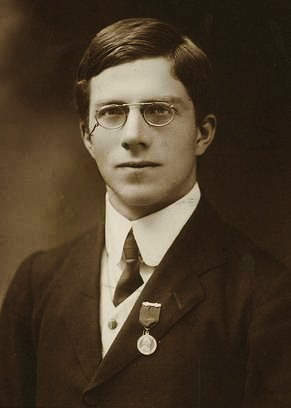
\includegraphics[width=3cm]{figures/fisher.jpg}
%\caption{Ronald Fisher (1890-1962)}
%\centering
%\end{figure}



\begin{columns}[T] % align columns
\begin{column}{.48\textwidth}

\vskip25pt

\small{

\begin{itemize}

\item Personalization is founded on the premise that individuals have heterogeneous responses to actions.
% the optimal action for person A and person B might be different. 

\vskip7pt

\item Personalization algorithms aim to improve decision-making by identifying and exploiting this heterogeneity.

\end{itemize}
}


\end{column}%
\hfill%


\begin{column}{.48\textwidth}


\begin{figure}[t]
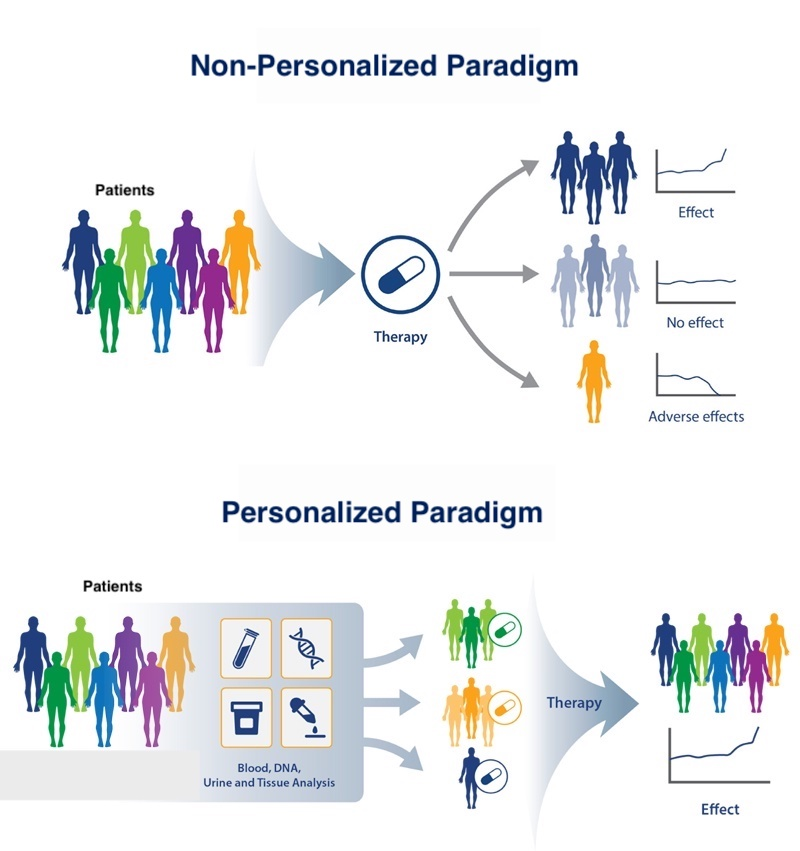
\includegraphics[width=5cm]{figures/personalizedmedv3.jpg}
\centering
\end{figure}


\end{column}%
\end{columns}


\end{frame}



%%%%Slide

\begin{frame}
[fragile]\frametitle{Unobserved and Heterogeneous Confounder (UHC)}



\begin{columns}[T] % align columns
\begin{column}{.48\textwidth}


\vskip15pt

\small{

\begin{itemize}

\item Treatment effect ($T$) varies according to the value of unobserved confounder/s ($U$).


\begin{equation*}
\begin{align*}
T:=& f(U) + N_T \\
Y :=& f(T, U, \boldsymbol{T \times U)} + N_Y
\end{align*}
\end{equation*}


\vskip7pt

\item Existence of UHCs is the most sensible assumption in practice. 
% the optimal action for person A and person B might be different. 


\vskip7pt

\item UHCs introduce challenges to personalization. 


\end{itemize}
}


\end{column}%

\begin{column}{.48\textwidth}


\vskip40pt

\begin{figure}
\begin{tikzpicture}
    \node[state, rectangle] (1) at (0,0)  {
\includegraphics[width=.20\textwidth]{figures/pill.png}};
    \node[state,  rectangle] (2) at (4, 0)  {$Y$};
    \node[state,  rectangle, dashed]  (3) at (2,1) {$U$};

    \path (1) edge  (2);
      \path[dashed] (3) edge  (1);
           \path[dashed] (3) edge  (2);
  \end{tikzpicture}
  
  \caption{Observational setting.}

\end{figure}


\end{column}%
\end{columns}

\end{frame}

%%%%Slide

\begin{frame}
[fragile]\frametitle{Motivating Questions}


Given the high-level goal of personalization, and the context of UHCs:

\vskip10pt

\begin{itemize}

\item Alternatives to how I formulate this problem? For instance, what is a suitable causal estimand?

\vskip7pt

\item What data do I need for identification? 

\vskip7pt

\item Is experimental data `gold standard'?

\end{itemize}

\vskip10pt

\textbf{Out-of-scope}: Estimation (e.g., compare different estimators). 


\end{frame}


%%%%Slide

\begin{frame}
[fragile]\frametitle{Motivating Example}

\begin{itemize}

\item \textbf{Business objective:}  Sell a credit card to new-to-RBC clients. 


\item \textbf{Current campaign}. All new-to-RBC clients who visited the RBC public site get a credit card offer $+$ iPad incentive.


\begin{figure}
   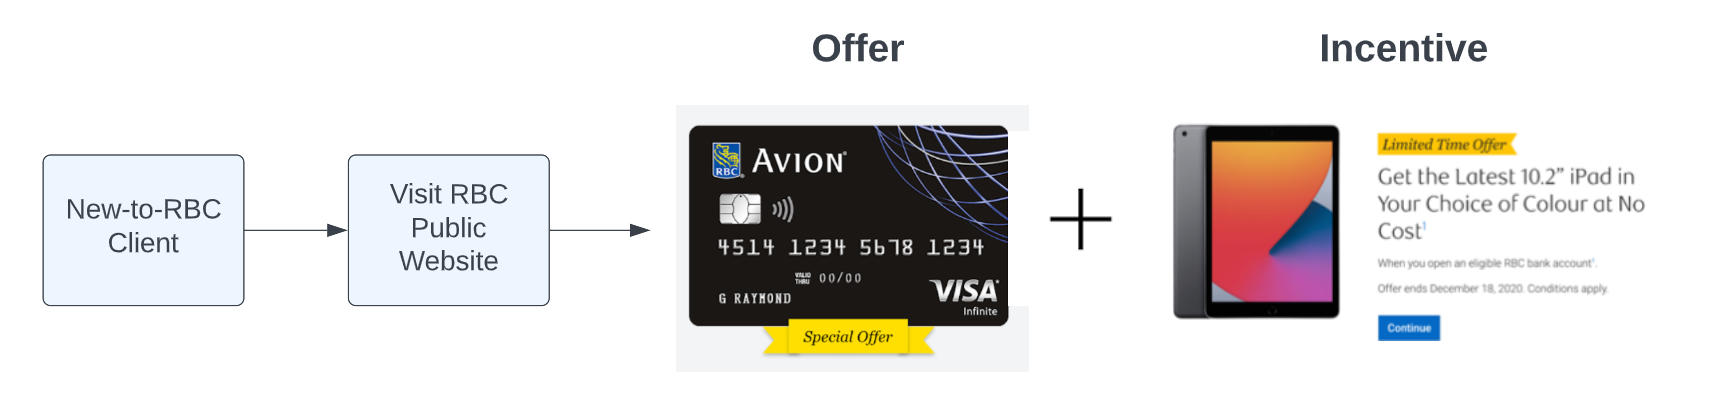
\includegraphics[width= 0.80\linewidth]{figures/campaign.png}
\end{figure}

\vskip20pt

\item \textbf{Business Goal: Personalize the incentive}. Identify which new-to-RBC clients should receive an iPad incentive in the future to maximize the expected profitability of the campaign. 

\end{itemize}

\end{frame}

%%%%Slide

\begin{frame}
[fragile]\frametitle{Data Generating Process}


\begin{columns}[T] % align columns
\begin{column}{.48\textwidth}

\begin{figure}
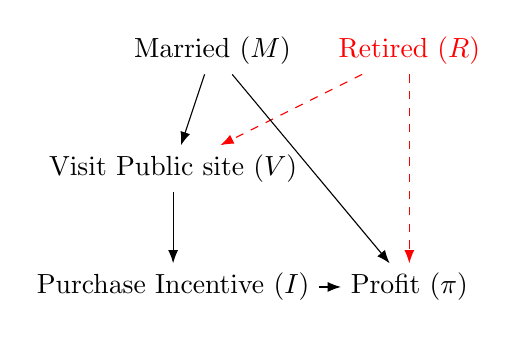
\begin{tikzpicture}
    \node (m) at (-0.5,0) {Married ($M$)};
    \node[red]  (r) at (2,0) {Retired ($R$)};
    \node (v) at (-1,-1.5) {Visit Public site ($V$)};
    \node (o) at (-1,-3) {Purchase Incentive ($I$)};
    \node (p) at (2,-3) {Profit ($\pi$)};

    \path (m) edge (v);
    \path[dashed, red] (r) edge (v);
     \path (m) edge (p);
     \path[dashed, red] (r) edge (p);
     \path (v) edge (o);
     \path (o) edge (p);
     
\end{tikzpicture}

\vskip 5pt

\caption{Observational setting.}

\end{figure}

\end{column}%
\hfill%

\pause

\begin{column}{.48\textwidth}

\vskip 20pt

\begin{equation*}
\begin{align*}
P(R=1)=&0.5~,~P(M=1)=0.5 \\
%P(m ,r)=& 0.25~\forall~m \in M, r \in R \\ 
V :=& M$\oplus$R  \\
I :=&  V 
\end{align*}
\end{equation*}
%}

\footnotesize{
\begin{table}
\begin{tabular}{ccccc}
\toprule
 &\multicolumn{2}{c}{$R=0$}
&
\multicolumn{2}{c}{$R=1$} \\\cmidrule(r){2-3}\cmidrule(l){4-5}
 & $M=1$ & $M=0$     & $M=1$ & $M=0$     \\  
 \midrule
$I=1$ &  \cellcolor{blue!25}{25} & 50 & 45 & \cellcolor{blue!25}{5} \\
$I=0$ &  50 & \cellcolor{blue!25}{10} & \cellcolor{blue!25}{5} & 30 \\
\bottomrule
\end{tabular}
\vskip5pt
\caption{$E[\pi|M, R, I]$. Highlighted cells reflect (new-to-RBC) client's 'natural' choice to visit the Public site or not.}
\end{table}
}


\end{column}%
\end{columns}
\end{frame}

%%%%Slide

\begin{frame}
[fragile]\frametitle{Four Approaches to Personalizing the Incentive}


\textbf{Business Goal}: Identify which new-to-RBC clients should receive an iPad incentive in the future to maximize the expected profitability of the campaign.

\vskip20pt

\begin{figure}[t]

\includegraphics[width=8cm]{figures/four.png}
\centering
\end{figure}

\end{frame}

%%%%Slide

\begin{frame}
[fragile]\frametitle{1. Associational Inference}

\begin{tikzpicture}[remember picture, overlay]
\node[left] at (current page.33) 
{
    
\includegraphics[width=0.1\textwidth]{figures/ds1.png}
};
\end{tikzpicture}

\begin{columns}[T] % align columns
\begin{column}{.48\textwidth}

\begin{center}
$\mathcal{D}^*_{\text{AI}}(M) = ~$\underset{I \in {0,1}}{\mathrm{argmax}}~E[\pi|I, M]$
\end{center}

\pause
\vskip10pt


\begin{equation*}
\begin{align*}
E[\pi | I=1, M=1] =& 25\\
E[\pi | I=0, M=1] =& 5\\
E[\pi | I=1, M=0] =& 5\\
E[\pi | I=0, M=0] =& 10 \\
\end{align*}
\end{equation*}


\end{column}%
\hfill%


\begin{column}{.48\textwidth}

\vskip 30pt

\footnotesize{
\begin{table}
 \begin{tabular}{ccccc}
\toprule
 &\multicolumn{2}{c}{$R=0$}
&
\multicolumn{2}{c}{$R=1$} \\\cmidrule(r){2-3}\cmidrule(l){4-5}
 & $M=1$ & $M=0$     & $M=1$ & $M=0$     \\  
 \midrule
$I=1$ &  \cellcolor{blue!25}{25} & 50 & 45 & \cellcolor{blue!25}{5} \\
$I=0$ &  50 & \cellcolor{blue!25}{10} & \cellcolor{blue!25}{5} & 30 \\
\bottomrule
\end{tabular}
\vskip5pt
\caption{$E[\pi|M, R, I]$.}
\end{table}
}



\end{column}%
\end{columns}

\vskip15pt

\pause

\textbf{Decision Rule}:

\small{
\begin{itemize}
\item If Visit Site $\land$ Married $\rightarrow$ Purchase Incentive $\rightarrow~E[\pi] = \textbf{25}  $
\item If Visit Site $\land$ Not Married $\rightarrow$ No Purchase Incentive  $\rightarrow~E[\pi] = \textbf{30} $
\end{itemize}
}

\vskip10pt

Expected profit = $\boxed{\mathbf{27.5}}$ = (25+30)/2.

\end{frame}


%%%%Slide

\begin{frame}
[fragile]\frametitle{2. Interventional Inference + Post-Visit Randomization}



\begin{tikzpicture}[remember picture, overlay]
\node[left] at (current page.33) 
{
    
\includegraphics[width=0.1\textwidth]{figures/ds2.png}
};
\end{tikzpicture}

\begin{columns}[T] % align columns
\begin{column}{.48\textwidth}

\begin{figure}
\begin{tikzpicture}[thick,scale=0.8, every node/.style={scale=0.8}]
    \node (m) at (-0.5,0) {Married ($M$)};
    \node[red]  (r) at (2,0) {Retired ($R$)};
    \node (v) at (-1,-1.5) {Visit Public site ($V$)};
    \node (o) at (-1,-3) {Purchase Incentive ($I$)};
    \node (p) at (2,-3) {Profit ($\pi$)};
    \node[blue] (c)  at (-4,-1.5) {Coin Flip ($C$)};

    \path (m) edge (v);
    \path[dashed, red] (r) edge (v);
     \path (m) edge (p);
     \path[dashed, red] (r) edge (p);
     \path (v) edge (o);
     \path (o) edge (p);
     \path[blue] (c) edge (o)
     
\end{tikzpicture}

\vskip 5pt

\caption{Causal DAG with post-visit randomization.}

\end{figure}

\end{column}%

\begin{column}{.48\textwidth}


\vskip 20pt

\begin{equation*}
\begin{align*}
V :=& M~$\oplus{}$ R  \\
I :=&  V \textcolor{blue}{\land C} 
\end{align*}
\end{equation*}


\end{column}%
\end{columns}

\end{frame}


%%%%Slide

\begin{frame}
[fragile]\frametitle{2. Interventional Inference + Post-Visit Randomization}

\begin{tikzpicture}[remember picture, overlay]
\node[left] at (current page.33) 
{
    
\includegraphics[width=0.1\textwidth]{figures/ds2.png}
};
\end{tikzpicture}


\begin{columns}[T] % align columns
\begin{column}{.55\textwidth}

\begin{center}
$\mathcal{D}^*_{\text{IPVR}}(M) = ~$\underset{I \in {0,1}}{\mathrm{argmax}}~E[\pi| do(I), M, V=1]$
\end{center}

\vskip10pt
\pause


\begin{equation*}
\begin{align*}
E[\pi | do(I=1), M=1, V=1] =& 25\\
E[\pi | do(I=0), M=1, V=1] =& 50\\
E[\pi | do(I=1), M=0, V=1] =& 5\\
E[\pi | do(I=0), M=0, V=1] =& 30
\end{align*}
\end{equation*}


\end{column}%
\hfill%


\begin{column}{.45\textwidth}

\vskip 30pt

\footnotesize{
\begin{table}
 \begin{tabular}{ccccc}
\toprule
 &\multicolumn{2}{c}{$R=0$}
&
\multicolumn{2}{c}{$R=1$} \\\cmidrule(r){2-3}\cmidrule(l){4-5}
 & $M=1$ & $M=0$     & $M=1$ & $M=0$     \\  
 \midrule
$I=1$ &  \cellcolor{blue!25}{25} & 50 & 45 & \cellcolor{blue!25}{5} \\
$I=0$ &  50 & \cellcolor{blue!25}{10} & \cellcolor{blue!25}{5} & 30 \\
\bottomrule
\end{tabular}
\vskip5pt
\caption{$E[\pi|M, R, I]$.}
\end{table}
}



\end{column}%
\end{columns}

\vskip15pt

\pause


\textbf{Decision Rule}:

\small{
\begin{itemize}
\item If Visit Site $\land$ Married $\rightarrow$ No Purchase Incentive $\rightarrow~E[\pi] = \textbf{50} $
\item If Visit Site $\land$ Not Married $\rightarrow$ No Purchase Incentive  $\rightarrow~E[\pi] = \textbf{30} $
\end{itemize}
}

\vskip10pt

Expected profit = $\boxed{\mathbf{40}}$ = (50+30)/2.



\end{frame}

%%%%Slide


\begin{frame}
[fragile]\frametitle{3. Interventional Inference + Full Randomization}

\begin{tikzpicture}[remember picture, overlay]
\node[left] at (current page.33) 
{
    
\includegraphics[width=0.1\textwidth]{figures/ds3.png}
};
\end{tikzpicture}

\begin{columns}[T] % align columns
\begin{column}{.48\textwidth}

\begin{figure}
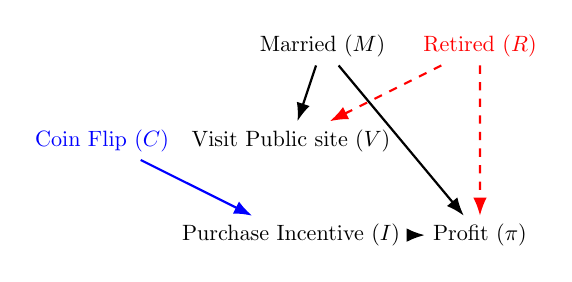
\begin{tikzpicture}[thick,scale=0.8, every node/.style={scale=0.8}]
    \node (m) at (-0.5,0) {Married ($M$)};
    \node[red]  (r) at (2,0) {Retired ($R$)};
    \node (v) at (-1,-1.5) {Visit Public site ($V$)};
    \node (o) at (-1,-3) {Purchase Incentive ($I$)};
    \node (p) at (2,-3) {Profit ($\pi$)};
    \node[blue] (c)  at (-4,-1.5) {Coin Flip ($C$)};

    \path (m) edge (v);
    \path[dashed, red] (r) edge (v);
     \path (m) edge (p);
     \path[dashed, red] (r) edge (p);
     \path (o) edge (p);
     \path[blue] (c) edge (o);
     
\end{tikzpicture}

\vskip 5pt
\begin{center}
\caption{Causal DAG with Full Randomization.}
\end{center}
\end{figure}

\end{column}%

\begin{column}{.48\textwidth}


\vskip 20pt

\begin{equation*}
\begin{align*}
V :=& M~$\oplus{}$ R  \\
I :=&  \textcolor{blue}{C} 
\end{align*}
\end{equation*}
%}

\end{column}%
\end{columns}




\end{frame}

%%%%Slide


\begin{frame}
[fragile]\frametitle{3. Interventional Inference + Full Randomization}

\begin{tikzpicture}[remember picture, overlay]
\node[left] at (current page.33) 
{
    
\includegraphics[width=0.1\textwidth]{figures/ds3.png}
};
\end{tikzpicture}

\begin{columns}[T] % align columns
\begin{column}{.48\textwidth}

\begin{center}
$\mathcal{D}^*_{\text{IFR}}(M) = ~$\underset{I \in {0,1}}{\mathrm{argmax}}~E[\pi|do(I), M]$
\end{center}

\vskip10pt

\scriptsize{
\begin{equation*}
\begin{align*}
E[\pi | do(I=1), M=1] &= 35.0=(25+45)/2 \\
E[\pi | do(I=0), M=1] &= 27.5 =(50 + 5)/2 \\
E[\pi | do(I=1), M=0] &= 27.5 =(50 + 5)/2 \\
E[\pi | do(I=0), M=0] &= 20.0 = (10 +30)/2 
\end{align*}
\end{equation*}
}


\end{column}%
\hfill%


\begin{column}{.48\textwidth}

\vskip30pt

\footnotesize{
\begin{table}
 \begin{tabular}{ccccc}
\toprule
 &\multicolumn{2}{c}{$R=0$}
&
\multicolumn{2}{c}{$R=1$} \\\cmidrule(r){2-3}\cmidrule(l){4-5}
 & $M=1$ & $M=0$     & $M=1$ & $M=0$     \\  
 \midrule
$I=1$ &  \cellcolor{blue!25}{25} & 50 & 45 & \cellcolor{blue!25}{5} \\
$I=0$ &  50 & \cellcolor{blue!25}{10} & \cellcolor{blue!25}{5} & 30 \\
\bottomrule
\end{tabular}
\vskip5pt
\caption{$E[\pi|M, R, I]$.}
\end{table}
}



\end{column}%
\end{columns}

\vskip15pt

\pause

\textbf{Decision Rule}:

\small{
\begin{itemize}
\item If  Married $\rightarrow$ Purchase Incentive $\rightarrow~E[\pi] = \textbf{35}  $
\item If  Not Married $\rightarrow$ Purchase Incentive  $\rightarrow~E[\pi] = \textbf{27.5} $
\end{itemize}
}

\vskip10pt

Expected profit = $\boxed{\mathbf{31.5}}$ = (35+27.5)/2.

\end{frame}

%%%%Slide

\begin{frame}
[fragile]\frametitle{4. Counterfactual Inference}

\begin{tikzpicture}[remember picture, overlay]
\node[left] at (current page.33) 
{
    
\includegraphics[width=0.1\textwidth]{figures/ds4.png}
};
\end{tikzpicture}

%\vskip-50pt

$\mathcal{D}^*_{\text{CI}}(M, I) = ~$\underset{a' \in~{0,1}}{\mathrm{argmax}}~E[\pi_{a'}| I=a, M]$

\pause

\vskip5pt

\begin{enumerate}

\item Do we need to assume a parametric model to identify this causal estimand?

\pause

\begin{itemize}

\item No. Only unit-level counterfactuals require a parametric model for identification.

\item There is nothing personal about personalization!

\end{itemize}

\pause

\vskip10pt

\item Do we need to assume that the conditioning set $\{M\}$ satisfies the \emph{backdoor criterion} to identify this causal estimand?

\pause

\begin{itemize}

\item In general, we do need to assume the conditioning set $Z=\{M\}$ satisfies the backdoor criterion. 

\item An exception is when $I$ is binary and both experimental and observational data are available. 

\end{itemize}

\end{enumerate}

\end{frame}

%%%%Slide

\begin{frame}
[fragile]\frametitle{4. Counterfactual Inference}

\begin{tikzpicture}[remember picture, overlay]
\node[left] at (current page.33) 
{
    
\includegraphics[width=0.1\textwidth]{figures/ds4.png}
};
\end{tikzpicture}

$\mathcal{D}^*_{\text{CI}}(M, I) = ~$\underset{a' \in~{0,1}}{\mathrm{argmax}}~E[\pi_{a'}| I=a, M]$

\vskip5pt

\scriptsize
\begin{equation*}
\begin{align*}
P(\pi_{a'}, M) &= P(\pi_{a'}, M, a') +  P(\pi_{a'}, M, a) \\
                      &=  P(\pi_{a'} | M, a') P(M, a') + P(\pi_{a'} | M, a) P(M, a) \\ \\
 P(\pi_{a'} | M)  &= P(\pi_{a'} | M, a') P( a' | M)  + P(\pi_{a'} | M, a) P(a | M) \\
                        &= P(\pi | M, a') P( a' | M)  + P(\pi_{a'} | M, a) P(a | M) ~\text{(Consistency)} \\ \\
P(\pi_{a'} | M, a) &= \frac{1}{P(a|M)} \Bigl[P(\pi_{a'} | M) -  P(\pi | M, a') P( a' | M) \Bigr] \\
&=\boxed{{\underbrace{\frac{1}{P(a|M)}}_{\text{\textcolor{blue}{observational}}}}   {\overbrace{ \Bigl[P\Big(\pi | M, do(a')\Big) }^{\text{\textcolor{blue}{experimental}}}} -  {\underbrace{ P(\pi | M, a') P( a' | M) \Bigr]}_{\text{\textcolor{blue}{observational}}}}}
\end{align*}
\end{equation*}

 %{\overbrace{ P(\pi | M, a') P( a' | M) \Bigr]}}^{\text{observational}}}
%  {\overbrace{ P(\pi | M, a') P( a' | M)  }^{\text{observational}}}

\end{frame}

%%%%Slide

\begin{frame}
[fragile]\frametitle{4. Counterfactual Inference}

\begin{tikzpicture}[remember picture, overlay]
\node[left] at (current page.33) 
{
    
\includegraphics[width=0.1\textwidth]{figures/ds4.png}
};
\end{tikzpicture}

\begin{columns}[T] % align columns
\begin{column}{.48\textwidth}

\begin{footnotesize}

$\boxed{E(\pi_{I=1} | M=1, I=0)} = $
\begin{equation*}
\begin{align*}
 \frac{1}{P(I=0|M=1)} \Bigl[E\Big(\pi | M=1, do(I=1)\Big) -  \\
 E(\pi | M=1, I=1) P( I=1 | M=1) \Bigr].  & \\
 = \frac{1}{1/2} (35-25  \times 1/2)  & = \textbf{45} \\
  > 5 = E(\pi_{I=0} | M=1, I=0).
\end{align*}
\end{equation*}

$\boxed{E(\pi_{I=1} | M=0, I=0)} = \textbf{50} \\ $ 

$\boxed{E(\pi_{I=0} | M=1, I=1)} = \textbf{50} \\ $ 

$\boxed{E(\pi_{I=0} | M=0, I=1)} = \textbf{30} \\ $ 

\end{footnotesize}


\end{column}%
\hfill%


\begin{column}{.48\textwidth}

\vskip30pt

\footnotesize{
\begin{table}
 \begin{tabular}{ccccc}
\toprule
 &\multicolumn{2}{c}{$R=0$}
&
\multicolumn{2}{c}{$R=1$} \\\cmidrule(r){2-3}\cmidrule(l){4-5}
 & $M=1$ & $M=0$     & $M=1$ & $M=0$     \\  
 \midrule
$I=1$ &  \cellcolor{blue!25}{25} & 50 & 45 & \cellcolor{blue!25}{5} \\
$I=0$ &  50 & \cellcolor{blue!25}{10} & \cellcolor{blue!25}{5} & 30 \\
\bottomrule
\end{tabular}
\vskip5pt
\caption{$E[\pi|M, R, I]$.}
\end{table}
}

\end{column}%
\end{columns}

\pause

\vskip5pt

\scriptsize{
\textbf{Decision Rule}:

\small{
\begin{itemize}
\item If Not Visit Site $\land$ Married $\rightarrow$ Purchase Incentive $\rightarrow~E[\pi] = \textbf{45} $
\item If Not Visit Site $\land$ Not Married $\rightarrow$ Purchase Incentive  $\rightarrow~E[\pi] = \textbf{50} $
\item If Visit Site $\land$ Married $\rightarrow$ No Purchase Incentive $\rightarrow~E[\pi] = \textbf{50} $
\item If Visit Site $\land$ Not Married $\rightarrow$ No Purchase Incentive  $\rightarrow~E[\pi] = \textbf{30} $
\end{itemize}
}


\vskip5pt

Expected profit = $\boxed{\mathbf{43.75}}$ = (45 + 50+ 50 +30)/4.
}

\end{frame}

%%%%Slide

\begin{frame}
[fragile]\frametitle{Summary of Methods}
\setlength{\leftmargini}{0pt}
\begin{table}[H]
   \label{tab:example}
   \scriptsize
   \centering
   \begin{tabular}{p{2cm} p{4cm} p{2cm} }
   \toprule
   \textbf{Criterion} & \textbf{Decision Rule} & $E[\pi] $ \\  
   \midrule
$\mathcal{D}_{AI}$ & 

\begin{itemize}
\item If Visit Site $\land$ Married $\rightarrow$ \textbf{Purchase Incentive} 
\item If Visit Site $\land$ Not Married $\rightarrow$ \textbf{No Purchase Incentive}
\end{itemize}

  
    
&  27.50 &\\ \hline
$\mathcal{D}_{IPVR}$& \textbf{Never Purchase Incentive} & 40.0 \\ \\ \hline
$\mathcal{D}_{IFR}$& \textbf{Always Purchase Incentive} &  31.50  \\ \\ \hline
$\mathcal{D}_{CI}$ & 

\begin{itemize}
\item If Visit Site $\land$ Married $\rightarrow$ \textbf{No Purchase Incentive} 
\item If Visit Site $\land$ Not Married $\rightarrow$ \textbf{No Purchase Incentive} 
\item If Not Visit Site $\land$ Married $\rightarrow$ \textbf{Purchase Incentive} 
\item If Not Visit Site $\land$ Not Married $\rightarrow$ \textbf{Purchase Incentive} 
\end{itemize}

& \textbf{43.75}  \\ \hline
$\mathcal{D}_{\text{Oracle}}$ & & \textbf{43.75} \\ \\ 
   \bottomrule
   \end{tabular}
\end{table}
\end{frame}


%%%%Slide

\begin{frame}
[fragile]\frametitle{Remarks}

\begin{itemize}

\item Experimental data are `gold standard' in the non-personalized paradigm because they remove the influence of unobserved confounders.

\vskip12pt

\item In the personalization paradigm, experimental data alone is not `gold standard' for estimating heterogeneous treatment effects in the presence of (UHCs).

\vskip12pt

\item Experiments `destroy' information that can be valuable to recover these confounders. 

\vskip12pt

\item Counterfactual-based decision-making for personalization leads to a fusion of experimental and observational data. 

\vskip12pt


\end{itemize}

\end{frame}

%%%%Slide


\begin{frame}
[fragile]\frametitle{Further Reading}

\begin{itemize}

\item The expression derived from RDC works only in the binary treatment case. 

\vskip5pt

\begin{itemize}
\item RDC-type randomization \href{https://proceedings.mlr.press/v70/forney17a.html}{(Forney et al., 2017) }
was proposed to estimate counterfactual expressions empirically from an arbitrary number of treatments. 
\end{itemize}

\vskip15pt

\item This presentation is fundamentally inspired by this paper: 

\vskip5pt

\begin{itemize}


\item Elias Bareinboim, Andrew Forney, and Judea Pearl. 2015. Bandits with unobserved confounders: a causal approach. In Proceedings of the 28th International Conference on Neural Information Processing Systems - Volume 1 (NIPS'15). 


\item Implementation: \url{https://github.com/leoguelman/mabuc}.

\end{itemize}


\end{itemize}

\end{frame}

\end{document}

